%\documentclass{beamer}
\documentclass[11pt,handout,pdf,hyperref={unicode}]{beamer}
\setbeamertemplate{navigation symbols}{}

\usepackage[T2A]{fontenc}
\usepackage[utf8]{inputenc}
\usepackage[english,russian]{babel}
\usepackage[style=authoryear]{biblatex}
\renewcommand*{\nameyeardelim}{\addcomma\addspace}
\graphicspath{ {images/} }
\DeclareGraphicsExtensions{.png,.pdf}
\addbibresource{custom.bib}
\usetheme{Warsaw}

\addtobeamertemplate{navigation symbols}{}{%
    \usebeamerfont{footline}%
    \usebeamercolor[black]{footline}%
    \hspace{10em}%
    \insertframenumber/\inserttotalframenumber
}

%Information to be included in the title page:
\title[Тайм-трекинг на блокчейне]{Тайм-трекинг пользовательских действий на распределенной блокчейн-цепи}

\begin{document}

\author[Михаил Волхов, M3438]{
  Студент: Михаил Волхов, M3438\\
  Руководитель: Штукенберг Д.Г., тьютор кафедры КТ \\
  Рецензцент: Чепурной А.И, специалист, IOHK Research
}
\institute{Кафедра Компьютерных Технологий \\ факультет Информационных Технологий и Программирования \\ Университет ИТМО, Санкт-Петербург}
\date{16 мая 2017}

\frame{\titlepage}

\section{Введение и цели}

\subsection{Блокчейн и криптовалюты}

\begin{frame}
  \frametitle{Блокчейн}

  Блок -- тело с данными и заголовок, содержащий подписанный ключом
  эмитентом хэш предыдущего блока. Объединяются так в цепочку. Право
  выпустить блок основывается на идее консенсуса:
  \begin{itemize}
  \item Proof-of-work (PoW): стохастически, решение сложной
    вычислительной задачи. Используется в Bitcoin \parencite{bitcoin}.
  \item Proof-of-stake (PoS): выбор лидера с вероятностью,
    пропорциональной его активам (stake).
  \end{itemize}

\end{frame}

\begin{frame}
  \frametitle{Криптовалюта}

  Тело блока содержит транзакции, переводящие средства с адресов на
  адреса. Адрес $Addr_i$ -- это хэш публичного ключа или скрипта. К
  транзакции прикладываются доказательства $\forall t \in txIn$.

  \begin{figure}[t]
  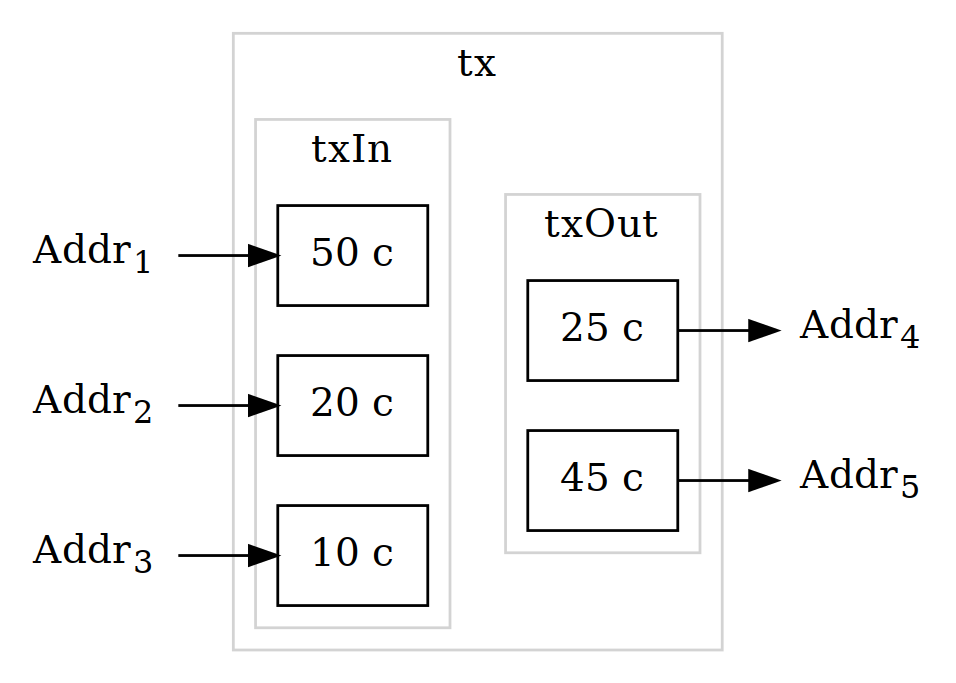
\includegraphics[scale=0.2]{tx_example}
  \centering
  \end{figure}
\end{frame}

\begin{frame}
  \frametitle{Скриптинг и смарт-контракты}

  Деньги могут храниться не только на адресе публичного ключа, но и на скрипте.
  \begin{itemize}
  \item Адрес -- хэш скрипта
  \item Сам скрипт говорит, как можно снимать со скрипт адреса деньги.
  \item Адреса, с которых может снимать $n/m$ пользователей (multisig)
  \item Смарт-контракты, например аукционы в Hawk \parencite{kosba2016hawk}
    или DAO (decentralized autonomous organisations) в Ethereum.
  \end{itemize}
\end{frame}


\begin{frame}
  \frametitle{Свойства Блокчейн-консенсуса}
  По сравнению с BFT алгоритмами \parencite{powbftquest}:
  \begin{itemize}
  \item Открытость по отношению к участникам, полная децентрализация.
  \item Отличное масштабирование по пользователям и узлам.
  \item Но меньшая производительность (из-за возможных форков).
  \end{itemize}

  Более оптимальное построения для публичных децентрализованных
  систем.
\end{frame}

\subsection{Тайм-трекинг}

\begin{frame}
  \frametitle{Тайм-трекинг и органайзеры}

  ПО, позволяющее ассоциировать активности с набором временных
  интервалов, а также анализировать эту статистику. Например, toggl,
  arbtt (автоматизированный, интеграция с X11) или org-mode.

  Пример тайм-трекинга задач в org-mode:
  \begin{figure}[t]
  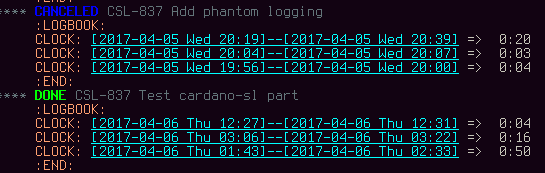
\includegraphics[scale=0.5]{org_mode_task}
  \centering
  \end{figure}
\end{frame}

\begin{frame}
  \frametitle{Открытые задачи}

  Что бы хотелось видеть:
  \begin{itemize}
  \item Мультипользовательские транзакции -- знание о том, что группа
    пользователей выполняет активность совместно. Реализаций не
    существует.
  \item Формализованный и автоматизированный сбор статистики (но можно
    руками org-mode'ом, например, считая потраченное время по
    категориям задач).
  \end{itemize}
\end{frame}

\subsection{Поставленная задача}

\begin{frame}
  \frametitle{Идея}

  \begin{itemize}
  \item Мультипользовательские транзакции -- почти транзакции
    криптовалюты. Можно выразить интервалы времени, тип
    активности. Необходимы подписи всех участников.
  \item Блокчейн хранит данные $\Rightarrow$ можно вычислять
    \textit{рейтинг} пользователей по статистике с помощью
    смарт-контрактов, формализация правила выставления рейтинга --
    \textit{контракт}.
  \item Рейтинг публичный, глобальный и финальный. Не зависит от
    имплементации.
  \end{itemize}
\end{frame}

\begin{frame}
  \frametitle{Задача и примеры}
  Задача: разработать модификацию криптовалюты:
  \begin{itemize}
  \item Имеет функциональность тайм-трекинга.
  \item Мультипользовательские транзакции и контракты, выставление рейтинга.
  \item Не нарушает гарантий криптовалюты.
  \end{itemize}

  Примеры использования:
  \begin{itemize}
    \item Аггрегация глобального рейтинга фрилансеров, поддерживающая
      несколько бирж.
    \item Оптимизация семейных отношений, обязанности и доказательства
      их (не)выполнения.
  \end{itemize}
\end{frame}

\section{Проделанная работа}

\subsection{База и модификации}

\begin{frame}
  \frametitle{Ouroboros и слоттинг}
  Почему именно ouroboros.
\end{frame}

\begin{frame}
  \frametitle{Граф покраски и валидация }

  Показать, чо за граф, как транзакцию валидировать через поток.
\end{frame}

\begin{frame}
  \frametitle{Реальная инстанциация}

  Предложил реальную схему, показал как и зачем. Показал, что ничего
  не сломается.
\end{frame}

\subsection{Система контрактов}

\begin{frame}
  \frametitle{Контракт, обязательства}

  Формализовал это.
\end{frame}

\begin{frame}
  \frametitle{Выставление рейтинга}

  Написал это через вектор Шепли, получилось прикольно и какие-то
  свойства есть.
\end{frame}

\begin{frame}
  \frametitle{Общая схема}

  Про скрипт и транзакцию обновления.
\end{frame}

\subsection{Инфраструктура}

\begin{frame}
  \frametitle{Проблема и логический слой}

  Что вообще за проблема, и вкратце про API.
\end{frame}

\begin{frame}
  \frametitle{Транспортный слой}

  Обзорчик на то, что можно и почему, показать какие проблемы возникают.
\end{frame}

\section{Результаты}

\begin{frame}
  \frametitle{Результаты}

  Спроектировал решение, получилось хорошо, всем требованиям удовлетворяет (показать).
\end{frame}

\section{}

\begin{frame}

  \begin{center}
    \Huge Вопросы?
  \end{center}

\end{frame}

\end{document}
